\chapter{Suunnittelu}
\label{ch:suunnittelu}
Tässä osuudessa käydään toteutetun ohjelman suunnittelu läpi ja kerrotaan miten ja miksi ratkaisuihin päädyttiin. Kappaleissa vertaillaan eri vaihtoehtoja ja peilataan demoversion ongelmia ja niiden perusteella yritetään löytää toimiva ratkaisu ongelmaan. Ensin suunnitellusta ohjelmasta annetaan kattava kokonaiskuva lukijalle ja tämän jälkeen tulevissa kappaleissa mennään jokaisen kohdan yksityiskohtiin tarkemmin.


\section{Kokonaiskuva}
Aikaisemmin kappaleessa \ref{ch:demoversio-ja-sen-toiminta} kuvassa \ref{fig:demo-architecture} esiteltiin demoversion arkkitehtuuri ja sen toiminta. Kuinka viestit IED-laitteelta kulkee ohjelman läpi ja tallennetaan tietokantaan. Tietokannasta muut ohjelmat lukevat tietoa kyselemällä sitä erikseen. Ongelmana tässä oli, että muut ohjelmat joutuivat kyselemään tietokannasta koko ajan, jos uusi viesti olisi saapunut. Suunnittelun jälkeen demoversion systeemistä päätyttiin kuvassa \ref{fig:planned-system-architecture} olevaan systeemin arkkitehtuuriin. Kuvassa katkoviivalla on merkitty tässä kappaleessa suunniteltu ohjelmisto. Ja kuvan yläreunassa oleva viiva kuvaa viestin kulkua järjestelmän eri osapuolten läpi ja missä muodossa viesti on missäkin kohtaa.

\begin{figure}
	\includegraphics[width=1\textwidth]{pictures/planned-system-architecture.png}
	\caption{Suunnitellun järjestelmän toiminta ja viestin kulkeminen ja muoto eri osapuolten välillä.}
	\label{fig:planned-system-architecture}
\end{figure}

Suunnitellussa arkkitehtuurissa C-kielellä toteutettu ohjelma voi tilata yhdellä IED-laitteella olevia RCB-instansseja. Tilattuaan RCB-instanssit, ohjelma odottaa viestejä IED-laitteelta IEC 61850 -standardin määrittämässä muodossa. Kun viesti saapuu, ohjelma prosessoi sen ja julkaisee AMPQ-standardin pohjaiselle jonopalvelimelle JSON-muodossa. Lopullisessa toteutuksessa jonopalvelimena käytettiin RabbitMQ-nimistä ohjelmistoa, joka pohjautuu AMPQ-standrdin versioon 0.9.1. Jonopalvelimelta muut tilaavat ohjelmat voivat tilata viestejä, ja viestin saapuessa palvelin ilmoittaa siitä asiakkaalle. Tällä vältetään jatkuva kyselyiden tekeminen ja tilaava ohjelman tarvitsee vain toimia kun viesti oikeasti saapuu. Lisäksi viestin uusi JSON-muoto on helppo lukea ihmiselle ja koneelle, eikä tilaavan asiakkaan tarvitse tehdä bittitason nypläystä. Toteutettu C-ohjelmisto käyttää edelleen demoversiosta tuttua libiec61850-kirjastoa hoitamaan matalan tason IEC 61850 -standardin määrittämän funktionaalisuuden.


\section{Järjestelmän hajautus ja arkkitehtuuri}
\begin{it}
	Lähde erilaisista hajautukista (pull vs pull, message queue) ja päätä mikä sopii tähän toteutukseen parhaiten ja miksi.
	Määritä ohjelman tarkempaa arkkitehtuuria mitä voidaan käyttää asetettujen ja yllämainittujen asioiden saavuttamiseen ja tarkentamiseen. Mitä jos käyttäjä tilaa monta viestiblokkia, niin missä järjestykssä asiat tehdään jne.
\end{it}


\section{Kielen valinta}
\begin{it}
	Kirjoita tähän kappaleeseen kielen valinnasta miksi tämä kieli otettiin. Kirjoita samalla että entisessä toteutuksessa kokeiltiin JRubya, missä ei ollut GILiä olemassa. Mikä tässä ei toiminut ja miksi siihen ei päädytty.
	Kirjoita miten kielen valinnalla myös parannetaan suorityskykyä paremmaksi.
\end{it}


\section{Ohjelmiston parametrisointi}
\begin{it}
	Kirjoita tähän ohjelmen parametrisoinnista ja miten ja miksi se tehtiin näin. Peilaa myös demon tietokannasta lukua mikä siinä ei ollut hyvä ja mitä tämä toteutus ratkaisee.
\end{it}


\section{Prosessoidun viestin muoto}
\begin{it}
	Kirjoita tähän mihin muotoon viestit lopussa tallennetaan esim. JSON. Miksi tähän valintaan päädyttiin. Kerro myös kuinka raportin alkuperäistä rakennetta muokattiin uuteen muotoon sopivaksi.
\end{it}